\documentclass[tikz,border=8pt]{standalone}
\usepackage{tikz}
\usetikzlibrary{positioning,arrows.meta}

\begin{document}
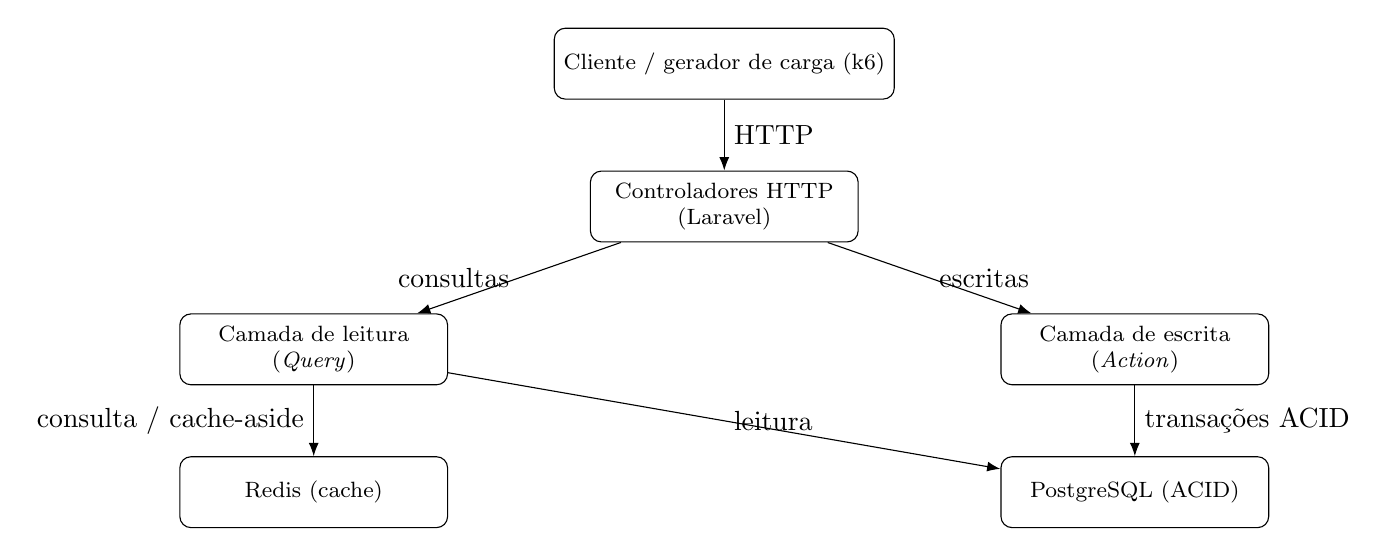
\begin{tikzpicture}[
    node distance=0.9cm and 1.8cm,
    >=Latex,
    box/.style={
        draw,
        rounded corners,
        align=center,
        minimum width=3.4cm,
        minimum height=0.9cm,
        font=\footnotesize
    }
]
    % Linha principal
    \node[box] (client) {Cliente / gerador de carga (k6)};
    \node[box, below=of client] (controller) {Controladores HTTP\\(Laravel)};

    % Split Query / Action
    \node[box, below left=of controller]  (query)  {Camada de leitura\\(\textit{Query})};
    \node[box, below right=of controller] (action) {Camada de escrita\\(\textit{Action})};

    % Armazenamento
    \node[box, below=of query]  (redis) {Redis (cache)};
    \node[box, below=of action] (pg)    {PostgreSQL (ACID)};

    % Setas principais
    \draw[->] (client) -- node[right]{HTTP} (controller);
    \draw[->] (controller) -- node[left]{consultas} (query);
    \draw[->] (controller) -- node[right]{escritas} (action);

    % Leitura: cache-aside
    \draw[->] (query) -- node[left]{consulta / cache-aside} (redis);
    \draw[->] (query) -- node[right]{leitura} (pg);

    % Escrita: só banco
    \draw[->] (action) -- node[right]{transações ACID} (pg);
\end{tikzpicture}
\end{document}
